% Source PDF page 229 (printed p. 215)
\section{拉格朗日对偶函数}
\subsection{拉格朗日函数}
考虑标准形式（4.1）的优化问题：
\begin{equation}
\begin{array}{ll}
\text{最小化}&f_0(x)\\
\text{约束为}&f_i(x)\le0,\quad i=1,\ldots,m\\
&h_i(x)=0,\quad i=1,\ldots,p,
\end{array}\tag{5.1}
\end{equation}
其中变量为 $x\in\R^n$。假设其定义域
$D=\bigcap_{i=0}^m\dom f_i\cap\bigcap_{i=1}^p\dom h_i$ 非空，并以 $p^\star$ 表示（5.1）的最优值。这里不假设问题（5.1）是凸的。

拉格朗日对偶的基本思想，是把约束函数的加权和加到目标函数中，从而将（5.1）的约束考虑在内。与问题（5.1）对应的\emph{拉格朗日函数} $L:\R^n\times\R^m\times\R^p\to\R$ 定义为
\[
L(x,\lambda,\nu)=f_0(x)+\sum_{i=1}^m\lambda_i f_i(x)
+\sum_{i=1}^p\nu_i h_i(x),
\]
其定义域为 $\dom L=D\times\R^m\times\R^p$。称 $\lambda_i$ 为对应于第 $i$ 个不等式约束 $f_i(x)\le0$ 的\emph{拉格朗日乘子}；类似地，称 $\nu_i$ 为对应于第 $i$ 个等式约束 $h_i(x)=0$ 的拉格朗日乘子。向量 $\lambda$ 和 $\nu$ 称为问题（5.1）的\emph{对偶变量}或\emph{拉格朗日乘子向量}。

% Source PDF page 230 (printed p. 216)
\subsection{拉格朗日对偶函数}
\emph{拉格朗日对偶函数}（简称\emph{对偶函数}）$g:\R^m\times\R^p\to\R$ 定义为拉格朗日函数关于 $x$ 的下确界：对于 $\lambda\in\R^m$、$\nu\in\R^p$，
\[
g(\lambda,\nu)=\inf_{x\in D}L(x,\lambda,\nu)
=\inf_{x\in D}\left(f_0(x)+\sum_{i=1}^m\lambda_i f_i(x)
+\sum_{i=1}^p\nu_i h_i(x)\right).
\]
当拉格朗日函数关于 $x$ 无下界时，对偶函数取值 $-\infty$。由于对偶函数是一族关于 $(\lambda,\nu)$ 的仿射函数的逐点下确界，因此即使问题（5.1）非凸，对偶函数也总是凹的。

\subsection{最优值的下界}
对偶函数给出问题（5.1）最优值 $p^\star$ 的下界：对于任意 $\lambda\succeq0$ 和任意 $\nu$，均有
\begin{equation}
g(\lambda,\nu)\le p^\star.\tag{5.2}
\end{equation}
这一重要性质很容易验证。设 $\widetilde x$ 是问题（5.1）的可行点，即 $f_i(\widetilde x)\le0$ 且 $h_i(\widetilde x)=0$，并设 $\lambda\succeq0$。此时
\[
\sum_{i=1}^m\lambda_i f_i(\widetilde x)+\sum_{i=1}^p\nu_i h_i(\widetilde x)\le0,
\]
因为第一个求和中的每一项都非正，第二个求和中的每一项都为零，所以
\[
L(\widetilde x,\lambda,\nu)
=f_0(\widetilde x)+\sum_{i=1}^m\lambda_i f_i(\widetilde x)
+\sum_{i=1}^p\nu_i h_i(\widetilde x)\le f_0(\widetilde x).
\]
因此
\[
g(\lambda,\nu)=\inf_{x\in D}L(x,\lambda,\nu)
\le L(\widetilde x,\lambda,\nu)\le f_0(\widetilde x).
\]
由于 $g(\lambda,\nu)\le f_0(\widetilde x)$ 对每个可行点 $\widetilde x$ 都成立，便得到不等式（5.2）。图5.1用一个 $x\in\R$、含一个不等式约束的简单问题说明了这个下界。

当 $g(\lambda,\nu)=-\infty$ 时，不等式（5.2）虽成立，却没有提供有效信息。只有当 $\lambda\succeq0$ 且 $(\lambda,\nu)\in\dom g$，即 $g(\lambda,\nu)>-\infty$ 时，对偶函数才给出 $p^\star$ 的非平凡下界。对于满足 $\lambda\succeq0$ 和 $(\lambda,\nu)\in\dom g$ 的 $(\lambda,\nu)$，称其为\emph{对偶可行}；这一名称的缘由稍后就会清楚。

\subsection{线性近似解释}
利用集合 $\{0\}$ 和 $-\R_+$ 的示性函数的线性近似，可以对拉格朗日函数及其下界性质作出简单解释。

% Source PDF page 231 (printed p. 217)
\begin{figure}[htbp]\centering
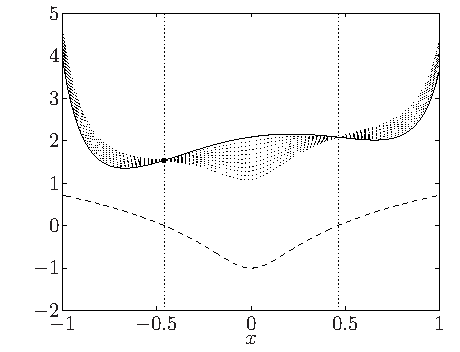
\includegraphics[width=.65\linewidth]{figures/ch05-fig01.pdf}
\caption*{图5.1\quad 对偶可行点给出的下界。实线表示目标函数 $f_0$，虚线表示约束函数 $f_1$。可行集是区间 $[-0.46,0.46]$，由两条点状竖线标出。最优点和最优值为 $x^\star=-0.46$、$p^\star=1.54$（以圆圈表示）。点线曲线表示 $\lambda=0.1,0.2,\ldots,1.0$ 时的 $L(x,\lambda)$。每条曲线的最小值都小于 $p^\star$，因为在可行集上（且 $\lambda\ge0$ 时），有 $L(x,\lambda)\le f_0(x)$。}
\end{figure}
\begin{figure}[htbp]\centering
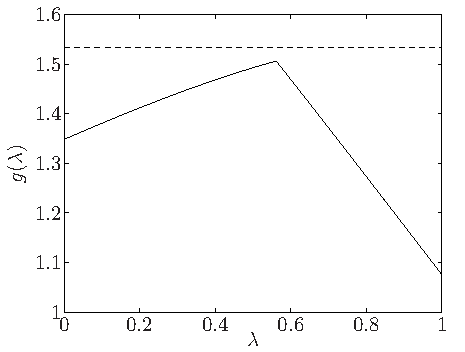
\includegraphics[width=.65\linewidth]{figures/ch05-fig02.pdf}
\caption*{图5.2\quad 图5.1中问题的对偶函数 $g$。虽然 $f_0$ 和 $f_1$ 都不是凸函数，但对偶函数是凹的。水平虚线表示问题的最优值 $p^\star$。}
\end{figure}

% Source PDF page 232 (printed p. 218)
首先把原问题（5.1）改写为无约束问题
\begin{equation}
\text{最小化}\quad f_0(x)+\sum_{i=1}^m I_-(f_i(x))
+\sum_{i=1}^p I_0(h_i(x)),\tag{5.3}
\end{equation}
其中 $I_-:\R\to\R$ 是非正实数集的示性函数，
\[
I_-(u)=\begin{cases}0&u\le0,\\ \infty&u>0,\end{cases}
\]
类似地，$I_0$ 是 $\{0\}$ 的示性函数。在表述（5.3）中，函数 $I_-(u)$ 可以理解为我们对约束函数值 $u=f_i(x)$ 的不满程度：若 $f_i(x)\le0$，不满为零；若 $f_i(x)>0$，不满为无穷大。同样，$I_0(u)$ 给出对等式约束值 $u=h_i(x)$ 的不满程度。可以把 $I_-$ 看作一道“砖墙”，或“无限硬”的不满函数：当 $f_i(x)$ 从非正变为正时，不满程度由零跃升至无穷大。

现在假设在（5.3）中，用线性函数 $\lambda_i u$（$\lambda_i\ge0$）代替 $I_-(u)$，用 $\nu_i u$ 代替 $I_0(u)$。目标就变成拉格朗日函数 $L(x,\lambda,\nu)$，对偶函数值 $g(\lambda,\nu)$ 是以下问题的最优值：
\begin{equation}
\text{最小化}\quad L(x,\lambda,\nu)=f_0(x)+\sum_{i=1}^m\lambda_i f_i(x)
+\sum_{i=1}^p\nu_i h_i(x).\tag{5.4}
\end{equation}
在这种表述中，我们用线性或“软”的不满函数代替 $I_-$ 和 $I_0$。对于不等式约束，当 $f_i(x)=0$ 时不满为零，而当 $f_i(x)>0$ 时不满为正（假设 $\lambda_i>0$）；约束违反得越多，不满程度就越大。在原来的表述中，$f_i(x)$ 的任意非正值都可以接受；在软表述中，有余量的约束，即 $f_i(x)<0$，实际上还会使我们感到满意。

显然，用线性函数 $\lambda_i u$ 近似示性函数 $I_-(u)$ 相当粗糙，但这个线性函数至少是示性函数的一个下估计。因为对任意 $u$ 都有 $\lambda_i u\le I_-(u)$ 和 $\nu_i u\le I_0(u)$，所以立即可知，对偶函数给出原问题最优值的一个下界。

用“软”版本代替“硬”约束的思想，在讨论内点法时还会再次出现（§11.2.1）。

\subsection{例子}
本节给出若干可以推导出拉格朗日对偶函数解析表达式的例子。

\subsubsection*{线性方程的最小二乘解}
考虑问题
\begin{equation}
\begin{array}{ll}\text{最小化}&x^\T x\\
\text{约束为}&Ax=b,\end{array}\tag{5.5}
\end{equation}
其中 $A\in\R^{p\times n}$。问题没有不等式约束，有 $p$ 个（线性）等式约束。拉格朗日函数为
$L(x,\nu)=x^\T x+\nu^\T(Ax-b)$，定义域为 $\R^n\times\R^p$。

% Source PDF page 233 (printed p. 219)
对偶函数为 $g(\nu)=\inf_x L(x,\nu)$。由于 $L(x,\nu)$ 是关于 $x$ 的凸二次函数，可由最优性条件
\[
\nabla_xL(x,\nu)=2x+A^\T\nu=0
\]
求得最小点 $x=-(1/2)A^\T\nu$。因此对偶函数为
\[
g(\nu)=L(-(1/2)A^\T\nu,\nu)=-(1/4)\nu^\T AA^\T\nu-b^\T\nu,
\]
这是定义域为 $\R^p$ 的凹二次函数。下界性质（5.2）说明，对于任意 $\nu\in\R^p$，都有
\[
-(1/4)\nu^\T AA^\T\nu-b^\T\nu\le\inf\{x^\T x\mid Ax=b\}.
\]

\subsubsection*{标准形式的线性规划}
考虑标准形式的线性规划
\begin{equation}
\begin{array}{ll}\text{最小化}&c^\T x\\
\text{约束为}&Ax=b\\&x\succeq0,\end{array}\tag{5.6}
\end{equation}
其不等式约束函数为 $f_i(x)=-x_i$，$i=1,\ldots,n$。为构造拉格朗日函数，对 $n$ 个不等式约束引入乘子 $\lambda_i$，对等式约束引入乘子 $\nu_i$，得到
\[
L(x,\lambda,\nu)=c^\T x-\sum_{i=1}^n\lambda_i x_i+\nu^\T(Ax-b)
=-b^\T\nu+(c+A^\T\nu-\lambda)^\T x.
\]
对偶函数为
\[
g(\lambda,\nu)=\inf_xL(x,\lambda,\nu)
=-b^\T\nu+\inf_x(c+A^\T\nu-\lambda)^\T x.
\]
由于线性函数只有在恒为零时才有下界，因此很容易解析地求出上式。除非 $c+A^\T\nu-\lambda=0$，否则 $g(\lambda,\nu)=-\infty$；等式成立时，其值为 $-b^\T\nu$：
\[
g(\lambda,\nu)=\begin{cases}
-b^\T\nu&A^\T\nu-\lambda+c=0,\\
-\infty&\text{其他情形}.
\end{cases}
\]
注意，对偶函数 $g$ 只在 $\R^m\times\R^p$ 的一个真仿射子集上为有限值。以后会看到，这种情况很常见。

下界性质（5.2）只有当 $\lambda,\nu$ 满足 $\lambda\succeq0$ 和 $A^\T\nu-\lambda+c=0$ 时才是非平凡的。这时 $-b^\T\nu$ 就是线性规划（5.6）最优值的下界。

\subsubsection*{二划分问题}
考虑（非凸）问题
\begin{equation}
\begin{array}{ll}\text{最小化}&x^\T Wx\\
\text{约束为}&x_i^2=1,\quad i=1,\ldots,n,\end{array}\tag{5.7}
\end{equation}

% Source PDF page 234 (printed p. 220)
其中 $W\in\mathbf S^n$。约束把 $x_i$ 的取值限制为 $1$ 或 $-1$，所以该问题等价于在所有分量为 $\pm1$ 的向量中，寻找使 $x^\T Wx$ 最小的一个。这里可行集是有限的（包含 $2^n$ 个点），因此原则上可以检查每个可行点的目标值来求解。不过，可行点数呈指数增长，这种方法仅适用于小问题（例如 $n\le30$）。一般而言（例如 $n$ 大于50时），问题（5.7）非常难解。

可将（5.7）解释为 $n$ 个元素（如 $\{1,\ldots,n\}$）的二划分问题：可行向量 $x$ 对应于划分
\[
\{1,\ldots,n\}=\{i\mid x_i=-1\}\cup\{i\mid x_i=1\}.
\]
矩阵系数 $W_{ij}$ 可以理解为将元素 $i,j$ 放在同一组的代价，$-W_{ij}$ 则是将二者放在不同组的代价。（5.7）的目标是对所有元素对求和得到的总代价，问题就是寻找总代价最小的划分。

现在推导其对偶函数。拉格朗日函数为
\begin{align*}
L(x,\nu)&=x^\T Wx+\sum_{i=1}^n\nu_i(x_i^2-1)\\
&=x^\T(W+\diag(\nu))x-\one^\T\nu.
\end{align*}
对 $x$ 最小化，得到拉格朗日对偶函数
\[
g(\nu)=\inf_x x^\T(W+\diag(\nu))x-\one^\T\nu
=\begin{cases}-\one^\T\nu&W+\diag(\nu)\succeq0,\\
-\infty&\text{其他情形},\end{cases}
\]
这里利用了二次型的下确界要么为零（当其半正定时），要么为 $-\infty$（当其非半正定时）。

这一对偶函数给出难解问题（5.7）最优值的下界。例如，可取对偶变量的特定值
\[
\nu=-\lambda_{\min}(W)\one.
\]
它是对偶可行的，因为 $W+\diag(\nu)=W-\lambda_{\min}(W)I\succeq0$。由此得到最优值 $p^\star$ 的界
\begin{equation}
p^\star\ge-\one^\T\nu=n\lambda_{\min}(W).\tag{5.8}
\end{equation}

\paragraph{注5.1}
也可以不借助拉格朗日对偶函数来得到这个下界。首先，用 $\sum_{i=1}^n x_i^2=n$ 代替约束 $x_1^2=1,\ldots,x_n^2=1$，得到修改后的问题
\begin{equation}
\begin{array}{ll}\text{最小化}&x^\T Wx\\
\text{约束为}&\sum_{i=1}^n x_i^2=n.\end{array}\tag{5.9}
\end{equation}

% Source PDF page 235 (printed p. 221)
原问题（5.7）的约束蕴含这里的约束，因此问题（5.9）的最优值是（5.7）最优值 $p^\star$ 的下界。而修改后的问题（5.9）容易作为特征值问题求解，其最优值为 $n\lambda_{\min}(W)$。

\subsection{拉格朗日对偶函数与共轭函数}
回顾§3.3，函数 $f:\R^n\to\R$ 的共轭 $f^*$ 为
\[
f^*(y)=\sup_{x\in\dom f}\bigl(y^\T x-f(x)\bigr).
\]
共轭函数与拉格朗日对偶函数密切相关。为说明一个简单联系，考虑问题
\[
\begin{array}{ll}\text{最小化}&f(x)\\\text{约束为}&x=0.\end{array}
\]
（这一问题并不十分有趣，观察即可求解。）其拉格朗日函数为 $L(x,\nu)=f(x)+\nu^\T x$，对偶函数为
\[
g(\nu)=\inf_x(f(x)+\nu^\T x)
=-\sup_x\bigl((-\nu)^\T x-f(x)\bigr)=-f^*(-\nu).
\]

更一般地（也更有用地），考虑带线性不等式和等式约束的优化问题
\begin{equation}
\begin{array}{ll}\text{最小化}&f_0(x)\\
\text{约束为}&Ax\preceq b\\&Cx=d.\end{array}\tag{5.10}
\end{equation}
利用 $f_0$ 的共轭，可将（5.10）的对偶函数写为
\begin{align}
g(\lambda,\nu)
&=\inf_x\bigl(f_0(x)+\lambda^\T(Ax-b)+\nu^\T(Cx-d)\bigr)\notag\\
&=-b^\T\lambda-d^\T\nu+\inf_x\bigl(f_0(x)+(A^\T\lambda+C^\T\nu)^\T x\bigr)\notag\\
&=-b^\T\lambda-d^\T\nu-f_0^*(-A^\T\lambda-C^\T\nu).\tag{5.11}
\end{align}
$g$ 的定义域可由 $f_0^*$ 的定义域得出：
\[
\dom g=\{(\lambda,\nu)\mid -A^\T\lambda-C^\T\nu\in\dom f_0^*\}.
\]
下面用几个例子说明。

\subsubsection*{等式约束范数最小化}
考虑问题
\begin{equation}
\begin{array}{ll}\text{最小化}&\norm{x}\\
\text{约束为}&Ax=b,\end{array}\tag{5.12}
\end{equation}

% Source PDF page 236 (printed p. 222)
其中 $\norm{\cdot}$ 是任意范数。回顾第93页的例3.26，$f_0=\norm{\cdot}$ 的共轭为
\[
f_0^*(y)=\begin{cases}0&\norm{y}_*\le1,\\
\infty&\text{其他情形},\end{cases}
\]
即对偶范数单位球的示性函数。利用上面的结果（5.11），问题（5.12）的对偶函数为
\[
g(\nu)=-b^\T\nu-f_0^*(-A^\T\nu)
=\begin{cases}-b^\T\nu&\norm{A^\T\nu}_*\le1,\\
-\infty&\text{其他情形}.\end{cases}
\]

\subsubsection*{熵最大化}
考虑熵最大化问题
\begin{equation}
\begin{array}{ll}\text{最小化}&f_0(x)=\sum_{i=1}^n x_i\log x_i\\
\text{约束为}&Ax\preceq b\\&\one^\T x=1,\end{array}\tag{5.13}
\end{equation}
其中 $\dom f_0=\R_{++}^n$。标量变量 $u$ 的负熵函数 $u\log u$ 的共轭为 $e^{v-1}$（见第91页例3.21）。由于 $f_0$ 是不同变量的负熵函数之和，可知其共轭为
\[
f_0^*(y)=\sum_{i=1}^n e^{y_i-1},\qquad \dom f_0^*=\R^n.
\]
利用结果（5.11），（5.13）的对偶函数为
\[
g(\lambda,\nu)=-b^\T\lambda-\nu-\sum_{i=1}^n e^{-a_i^\T\lambda-\nu-1}
=-b^\T\lambda-\nu-e^{-\nu-1}\sum_{i=1}^n e^{-a_i^\T\lambda},
\]
其中 $a_i$ 是 $A$ 的第 $i$ 列。

\subsubsection*{最小体积覆盖椭球}
考虑变量为 $X\in\mathbf S^n$ 的问题
\begin{equation}
\begin{array}{ll}\text{最小化}&f_0(X)=\log\det X^{-1}\\
\text{约束为}&a_i^\T Xa_i\le1,\quad i=1,\ldots,m,\end{array}\tag{5.14}
\end{equation}
其中 $\dom f_0=\mathbf S_{++}^n$。问题（5.14）有简单的几何解释。每个 $X\in\mathbf S_{++}^n$ 对应一个以原点为中心的椭球
\[
\mathcal E_X=\{z\mid z^\T Xz\le1\}.
\]
这个椭球的体积与 $(\det X^{-1})^{1/2}$ 成正比，所以除去一个常数和一个二倍因子，（5.14）的目标就是椭球体积的对数。

% Source PDF page 237 (printed p. 223)
问题（5.14）的约束要求 $a_i\in\mathcal E_X$。因此，它寻找包含点 $a_1,\ldots,a_m$、以原点为中心的最小体积椭球。

问题（5.14）的不等式约束是仿射的，可写为 $\tr((a_i a_i^\T)X)\le1$。在第92页例3.23中，已求得 $f_0$ 的共轭为
\[
f_0^*(Y)=\log\det(-Y)^{-1}-n,\qquad \dom f_0^*=-\mathbf S_{++}^n.
\]
利用结果（5.11），问题（5.14）的对偶函数为
\begin{equation}
g(\lambda)=\begin{cases}
\log\det\left(\sum_{i=1}^m\lambda_i a_i a_i^\T\right)-\one^\T\lambda+n
&\sum_{i=1}^m\lambda_i a_i a_i^\T\succ0,\\
-\infty&\text{其他情形}.
\end{cases}\tag{5.15}
\end{equation}
因此，对于任意满足 $\lambda\succeq0$、$\sum_{i=1}^m\lambda_i a_i a_i^\T\succ0$ 的 $\lambda$，
\[
\log\det\left(\sum_{i=1}^m\lambda_i a_i a_i^\T\right)-\one^\T\lambda+n
\]
都是问题（5.14）最优值的一个下界。

\section{拉格朗日对偶问题}
对于每个满足 $\lambda\succeq0$ 的 $(\lambda,\nu)$，拉格朗日对偶函数都给出优化问题（5.1）最优值 $p^\star$ 的一个下界。这样就有了一个依赖参数 $\lambda,\nu$ 的下界。自然要问：从拉格朗日对偶函数出发，能得到的最佳下界是什么？

由此得到优化问题
\begin{equation}
\begin{array}{ll}\text{最大化}&g(\lambda,\nu)\\
\text{约束为}&\lambda\succeq0.\end{array}\tag{5.16}
\end{equation}
这一问题称为问题（5.1）的\emph{拉格朗日对偶问题}。在这一语境中，原来的问题（5.1）有时称为\emph{原始问题}。现在，用“对偶可行”来描述满足 $\lambda\succeq0$ 和 $g(\lambda,\nu)>-\infty$ 的 $(\lambda,\nu)$ 就顺理成章了：它表示 $(\lambda,\nu)$ 是对偶问题（5.16）的可行点。若 $(\lambda^\star,\nu^\star)$ 是（5.16）的最优解，就称其为\emph{对偶最优解}或\emph{最优拉格朗日乘子}。

拉格朗日对偶问题（5.16）是凸优化问题，因为要最大化的目标是凹函数，约束也是凸的。无论原始问题（5.1）是否凸，这一点都成立。

% Source PDF page 238 (printed p. 224)
\subsection{显式写出对偶约束}
上面的例子说明，对偶函数的定义域
\[
\dom g=\{(\lambda,\nu)\mid g(\lambda,\nu)>-\infty\}
\]
的维数小于 $m+p$ 并不少见。许多情况下，可以确定 $\dom g$ 的仿射包，并把它描述为一组线性等式约束。粗略地说，就是可以识别出“隐藏”或“隐含”在对偶问题（5.16）目标 $g$ 中的等式约束。这时可以构造一个等价问题，将这些等式明确地列为约束。下面的例子说明这一思想。

\subsubsection*{标准形式线性规划的拉格朗日对偶}
第219页已求得标准形式线性规划
\begin{equation}
\begin{array}{ll}\text{最小化}&c^\T x\\
\text{约束为}&Ax=b\\&x\succeq0\end{array}\tag{5.17}
\end{equation}
的拉格朗日对偶函数为
\[
g(\lambda,\nu)=\begin{cases}-b^\T\nu&A^\T\nu-\lambda+c=0,\\
-\infty&\text{其他情形}.\end{cases}
\]
严格地说，标准形式线性规划的拉格朗日对偶问题是在 $\lambda\succeq0$ 上最大化上述 $g$，即
\begin{equation}
\begin{array}{ll}
\text{最大化}&g(\lambda,\nu)=
\begin{cases}-b^\T\nu&A^\T\nu-\lambda+c=0,\\-\infty&\text{其他情形}\end{cases}\\
\text{约束为}&\lambda\succeq0.
\end{array}\tag{5.18}
\end{equation}
只有当 $A^\T\nu-\lambda+c=0$ 时，$g$ 才是有限的。将这些等式约束显式写出，可得等价问题
\begin{equation}
\begin{array}{ll}\text{最大化}&-b^\T\nu\\
\text{约束为}&A^\T\nu-\lambda+c=0\\&\lambda\succeq0.\end{array}\tag{5.19}
\end{equation}
它又可表示为
\begin{equation}
\begin{array}{ll}\text{最大化}&-b^\T\nu\\
\text{约束为}&A^\T\nu+c\succeq0,\end{array}\tag{5.20}
\end{equation}
这是不等式形式的线性规划。

注意这三个问题之间的细微区别。标准形式线性规划（5.17）的拉格朗日对偶是（5.18），它与（5.19）、（5.20）等价，却并非同一个问题。稍微放宽术语，我们也将（5.19）或（5.20）称为标准形式线性规划（5.17）的拉格朗日对偶。
